\documentclass[12pt]{article}

% Ћирилица: кодирање фонта и језик (српски, ћирилица)
\usepackage[T2A]{fontenc}
\usepackage[utf8]{inputenc}
\usepackage[serbianc]{babel}

% Величина стране и маргине
\usepackage[a4paper,top=2cm,bottom=2cm,left=2.5cm,right=2.5cm]{geometry}

% Корисни пакети
\usepackage{amsmath}
\usepackage{enumitem}
\usepackage{float}
\usepackage{booktabs}
\usepackage{tcolorbox}
\tcbuselibrary{breakable}
\usepackage[colorlinks=true, allcolors=blue]{hyperref}

% Цртање електричних кола (европски симболи)
\usepackage[european]{circuitikz}
\usetikzlibrary{babel}

% Оквир за решене примере
\newtcolorbox[auto counter]{primer}{breakable,
    colback=white, colframe=black!55, colbacktitle=black!55, coltitle=white,
    fonttitle=\bfseries\small, title={Пример~\thetcbcounter},
    boxrule=0.5pt, arc=1.5pt, left=6pt, right=6pt, top=3pt, bottom=3pt,
    before skip=8pt, after skip=10pt}

% Оквир за кључне формуле
\newtcolorbox{kljucno}{colback=blue!4, colframe=blue!45!black,
    boxrule=0.5pt, arc=1.5pt, left=8pt, right=8pt, top=4pt, bottom=4pt}

\title{L/LH - Jetronic систем убризгавања - пропитивање}
\author{Аутоелектронски системи 2}
\date{}

\begin{document}
\maketitle


\section{L-Jetronic систем убризгавања}

L-Jetronic је потпуно електронски систем убризгавања. Слово L потиче од
немачке речи \textit{Luft} (ваздух), јер се количина горива одређује према
измереној количини усисаног ваздуха. Систем је настао као модификација
D-Jetronic система.

За разлику од K/KE-Jetronic-а, гориво се не убризгава непрекидно, већ у
импулсима. Свака бризгаљка је електромагнетни вентил који отвара управљачка
јединица. Притисак горива је сталан, па количина убризганог горива зависи само
од тога колико дуго је бризгаљка отворена.

\begin{figure}[H]
    \centering
    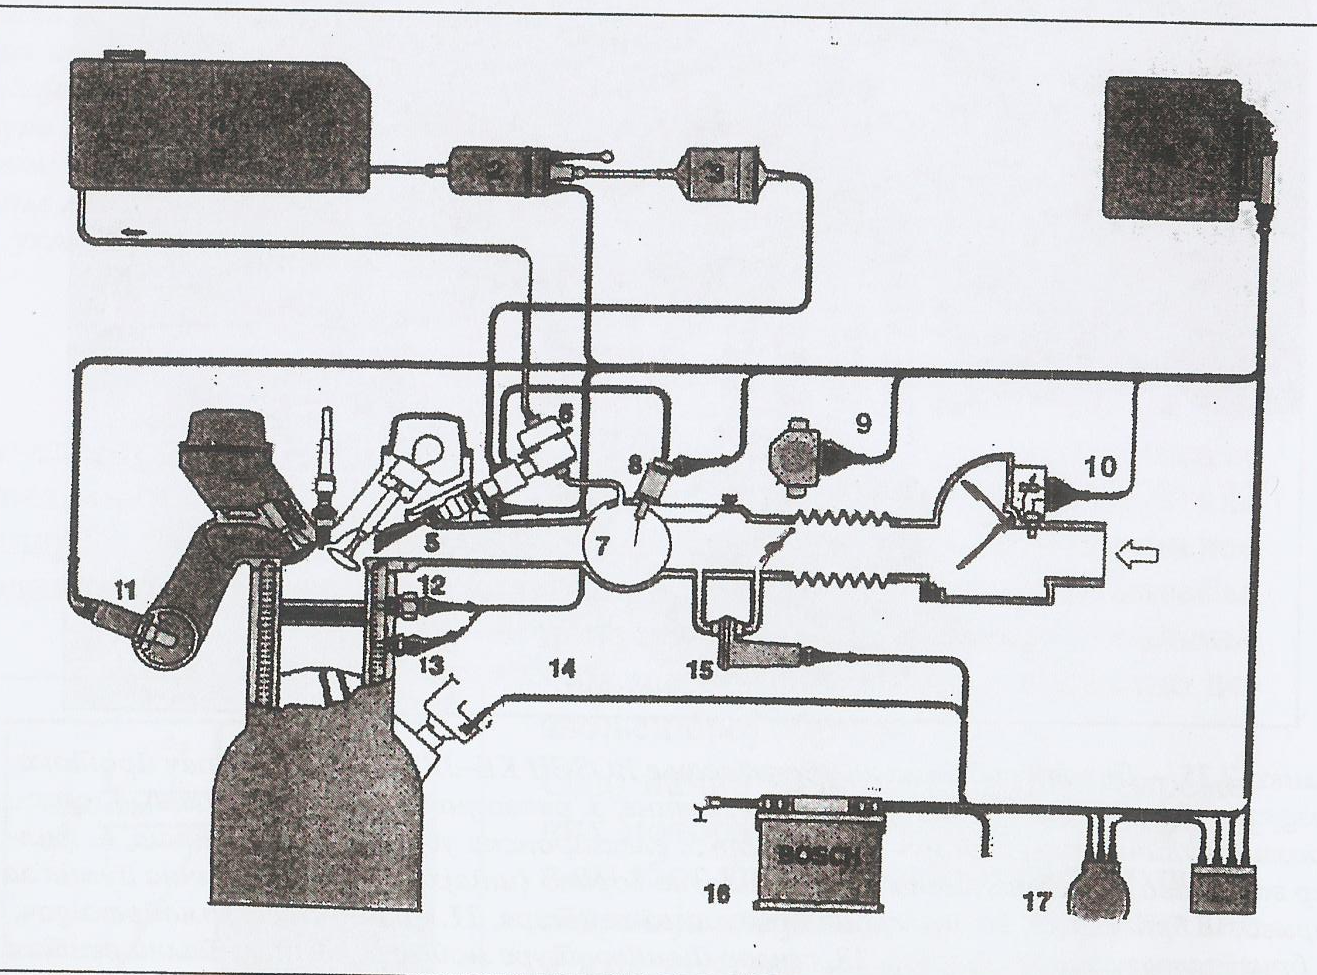
\includegraphics[width=0.7\textwidth]{slike/Le12.png}
    \caption{Шема система}
    \label{fig:primer}
\end{figure}

\begin{enumerate}
    \item[1.] Резервоар за гориво - место са бензином
    \item[2.] Електрична пумпа за гориво - потискивање горива под притиском
    \item[3.] Филтер за гориво - пречишћавање горива
    \item[4.] Електронска управљачка јединица - рачуна време убризгавања
    \item[5.] Бризгаљка - електромагнетни вентил за убризгавање
    \item[6.] Разводна цев са регулатором притиска - довод горива до бризгаљки под сталним притиском
    \item[7.] Усисни колектор - развод ваздуха до цилиндара
    \item[8.] Бризгаљка хладног старта - додатно гориво при хладном старту
    \item[9.] Прекидач пригушног лептира - сигнал празног хода и пуног оптерећења
    \item[10.] Мерач протока ваздуха (протокомер) - мерење усисаног ваздуха
    \item[11.] ЛАМБДА сонда - сензор мешавине
    \item[12.] Временски термопрекидач - укључивање бризгаљке хладног старта
    \item[13.] Сензор температуре мотора
    \item[14.] Разводник паљења - сигнал броја обртаја
    \item[15.] Биметални вентил у заобилазном воду - додатни ваздух за хладан мотор
    \item[16.] Акумулатор
    \item[17.] Контакт-кључ
\end{enumerate}

L-Jetronic систем се може поделити на три функционалне групе: 
\textbf{инсталација за напајање горивом}, \textbf{прикупљање и обрада података о мотору},
\textbf{регулација убризгавања количине горива}.

\subsection{Мерење количине усисаног ваздуха}

Мерење протока ваздуха је у случају L-Jetronic система потпуно електронска,
односно преко сензора.

\begin{figure}[H]
    \centering
    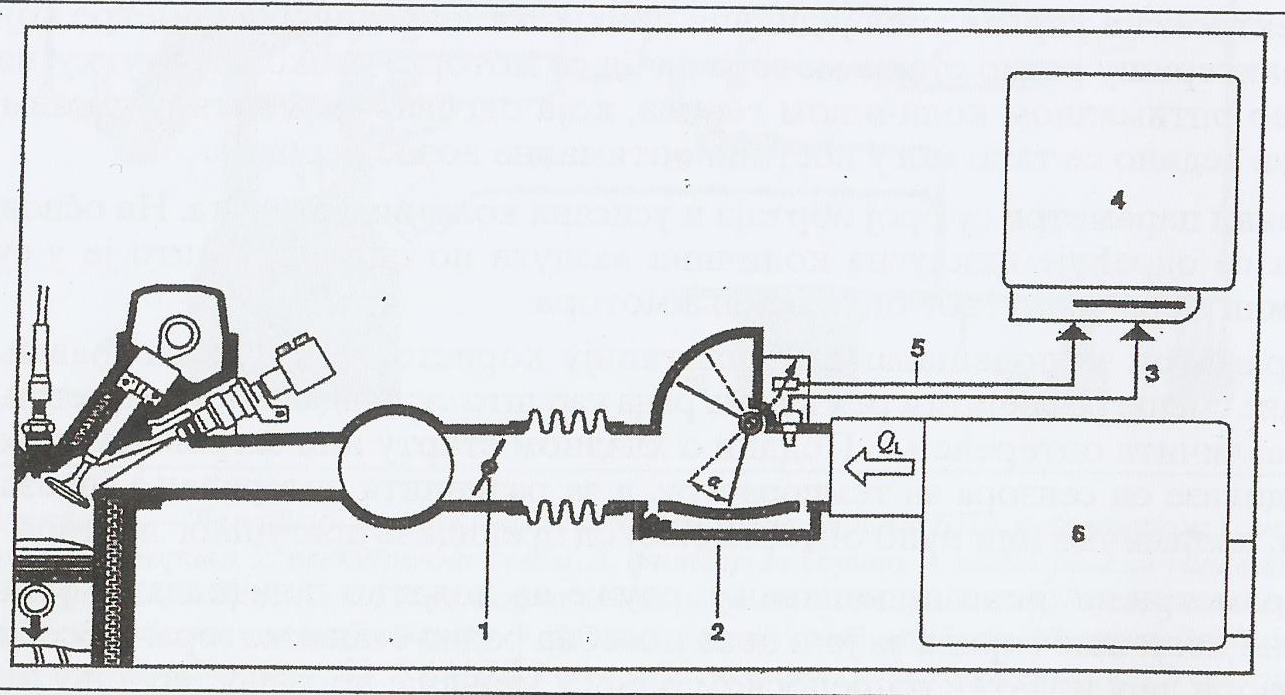
\includegraphics[width=0.4\textwidth]{slike/Le4.png}
    \caption{Мерење количине усисаног ваздуха}
    \label{fig:primer}
\end{figure}

Сензор који мери проток ваздуха назвамо \textbf{мерач протока ваздуха}
односно \textbf{протокомер}, исто као код КЕ система.

Сав усисни ваздух пролази кроз мерач. У њему је заклопка која се у струји
ваздуха закреће насупрот спиралној опрузи. Што је више ваздуха, заклопка се
више закрене. На њеној осовини је потенциометар, који управљачкој јединици
шаље напон сразмеран количини ваздуха.

Компензациона заклопка у пригушној комори смирује осцилације мерне заклопке.
Заобилазни канал са завртњем служи за подешавање састава смеше у празном ходу.

У мерачу су још:
\begin{itemize}
    \item \textbf{сензор температуре ваздуха} (Температурно зависни отпорник), јер топлији ваздух има
          мању густину, па му одговара мање горива,
    \item \textbf{контакт за пумпу}, који укључује пумпу само када ваздух
          струји, тј. када мотор ради.
\end{itemize}

\subsection{Прилагођавање радне смеше условима рада}

Прилагођавање смеше врши се помоћу компоненти: \textbf{прекидач пригушног лептира},\textbf{сензор температуре мотора}
, \textbf{ЛАМБДА регулатора}


\textbf{Прекидач пригушног лептира} остављен је на осовину пригушног лептира. Има контакт празног хода и контакт
пуног оптерећења, па управљачка јединица зна када је лептир затворен, а када
потпуно отворен.

\textbf{Сензор температуре мотора}је заправо 
емпературно зависни отпорник у облику сонде, увијен у блок мотора, са врхом у расхладној
течности. Јавља управљачкој јединици колико је мотор загрејан.

\textbf{ЛАМБДА регулација} врши се на основу сигнала од \textbf{ламбда сонде}. 
На основу одступања од идеалног случаја
ЕУЈ додатно коригује састав радне смеше, тако да средња вредност увек буде биска идеалном случају. 

\begin{figure}[H]
    \centering
    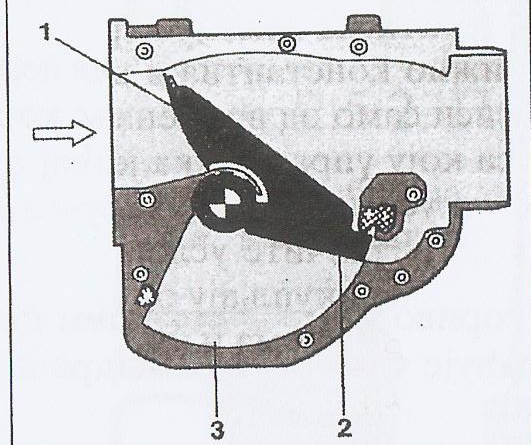
\includegraphics[width=0.4\textwidth]{slike/Le81.png}
    \caption{Ламбда регулатор}
    \label{fig:primer}
\end{figure}

\subsection{Електромагнетне бризгаљке}
 
За разлику од КЕ система, бризгаљке у L системима се контролишу електронски, на жељени такт.
Свака бризгаљка има намотај и иглу коју држи опруга. Када управљачка јединица
пусти струју кроз намотај, електромагнет подигне иглу и бризгаљка се отвори.
Када струја престане, опруга затвори иглу. Бризгаљка је отворена свега
неколико милисекунди.

%------------------------------------------------------------------
\section{LH-Jetronic}
%------------------------------------------------------------------

\begin{figure}[H]
    \centering
    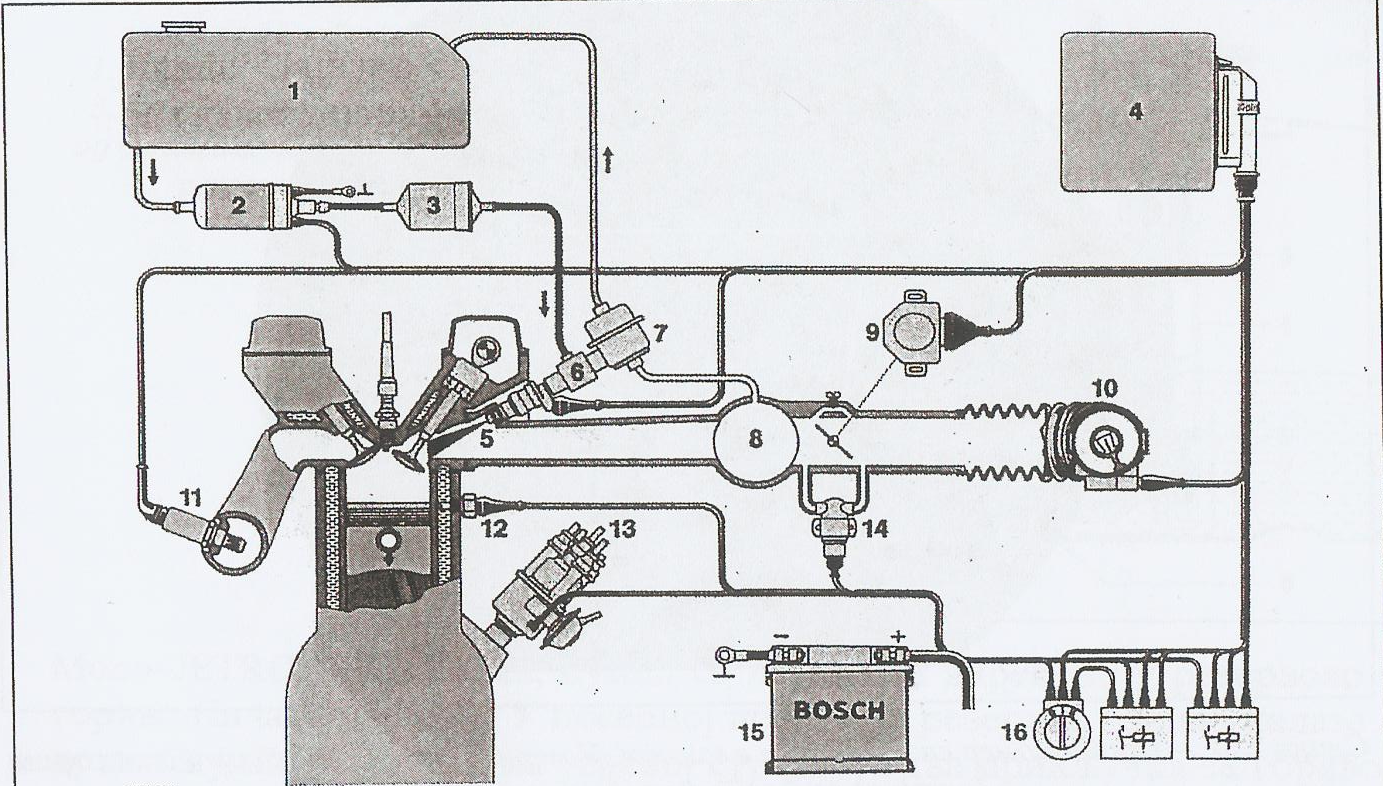
\includegraphics[width=0.8\textwidth]{slike/Le8.png}
    \caption{Шема LH-Jetronic система са компонентама}
    \label{fig:primer}
\end{figure}

LH-Jetronic је даљи развој L-Jetronic-а. Ознака LH потиче од \textit{Luft}
и \textit{Hitzdraht} (ваздух и врућа жица). Главна разлика је мерач: уместо
заклопке, која мери запремину ваздуха, користи се мерач који директно мери
масу ваздуха.

\subsection{Мерач масе ваздуха са врућом жицом}

У струји ваздуха разапета је танка платинска жица. Електроника је држи на
сталној температури, вишој од температуре ваздуха. Што више ваздуха протиче,
жица се више хлади и потребна је јача струја да остане загрејана. Јачина те
струје је мера масе усисаног ваздуха.

Предности у односу на заклопку:
\begin{itemize}
    \item Маса ваздуха већ обухвата његову температуру и притисак, па нису
          потребне корекције за температуру ваздуха и надморску висину,
    \item Нема покретних делова,
    \item Мањи је отпор струјању ваздуха,
    \item Мерач брже реагује на промене.
\end{itemize}

На жици се временом таложе нечистоће, које мењају мерење. Зато се после
гашења мотора жица накратко (око 1 секунду) загреје на високу температуру, па
наслаге изгоре.


\end{document}